\begin{tcolorbox}
\chapter{2012 - Sledi Vetra}

Sledi Vetra 2012 was a clear success. 2703 m of new cave passage was
found, the majority of which was below -600 m, once again using Camp
\passage{X-Ray} at -550 m as a base. The main discoveries in
\passage{Vrtnarija} include: the \passage{Watership Down} series below
\passage{Daydreamers}, adding 12 m of depth to the cave and taking it to -900 m;
about 1 km of horizontal development below \passage{Stuck in Paradise}
(-700 m); and the \passage{Apollo} extensions leading off a bolt climb in
the \passage{Queen's Bedchamber}. The \passage{Apollo} extensions also ended
up connecting to \passage{Waterloo} in \passage{System Migovec}, giving us the long
sought after connection and tying in \textasciitilde 15 years of
exploration by ICCC on \passage{Migovec}. \passage{System Migovec} is now 25592 m long, 973
m deep and has the distinction of being the longest cave in Slovenia.

Sledi Vetra was named to complement to Vodna Sled (Following / Stalking the Water) -- meaning Follow the Wind.

\end{tcolorbox}
\backgroundsetup{
    scale=1,
    color=black,
    opacity=1,
    angle=0,
    contents={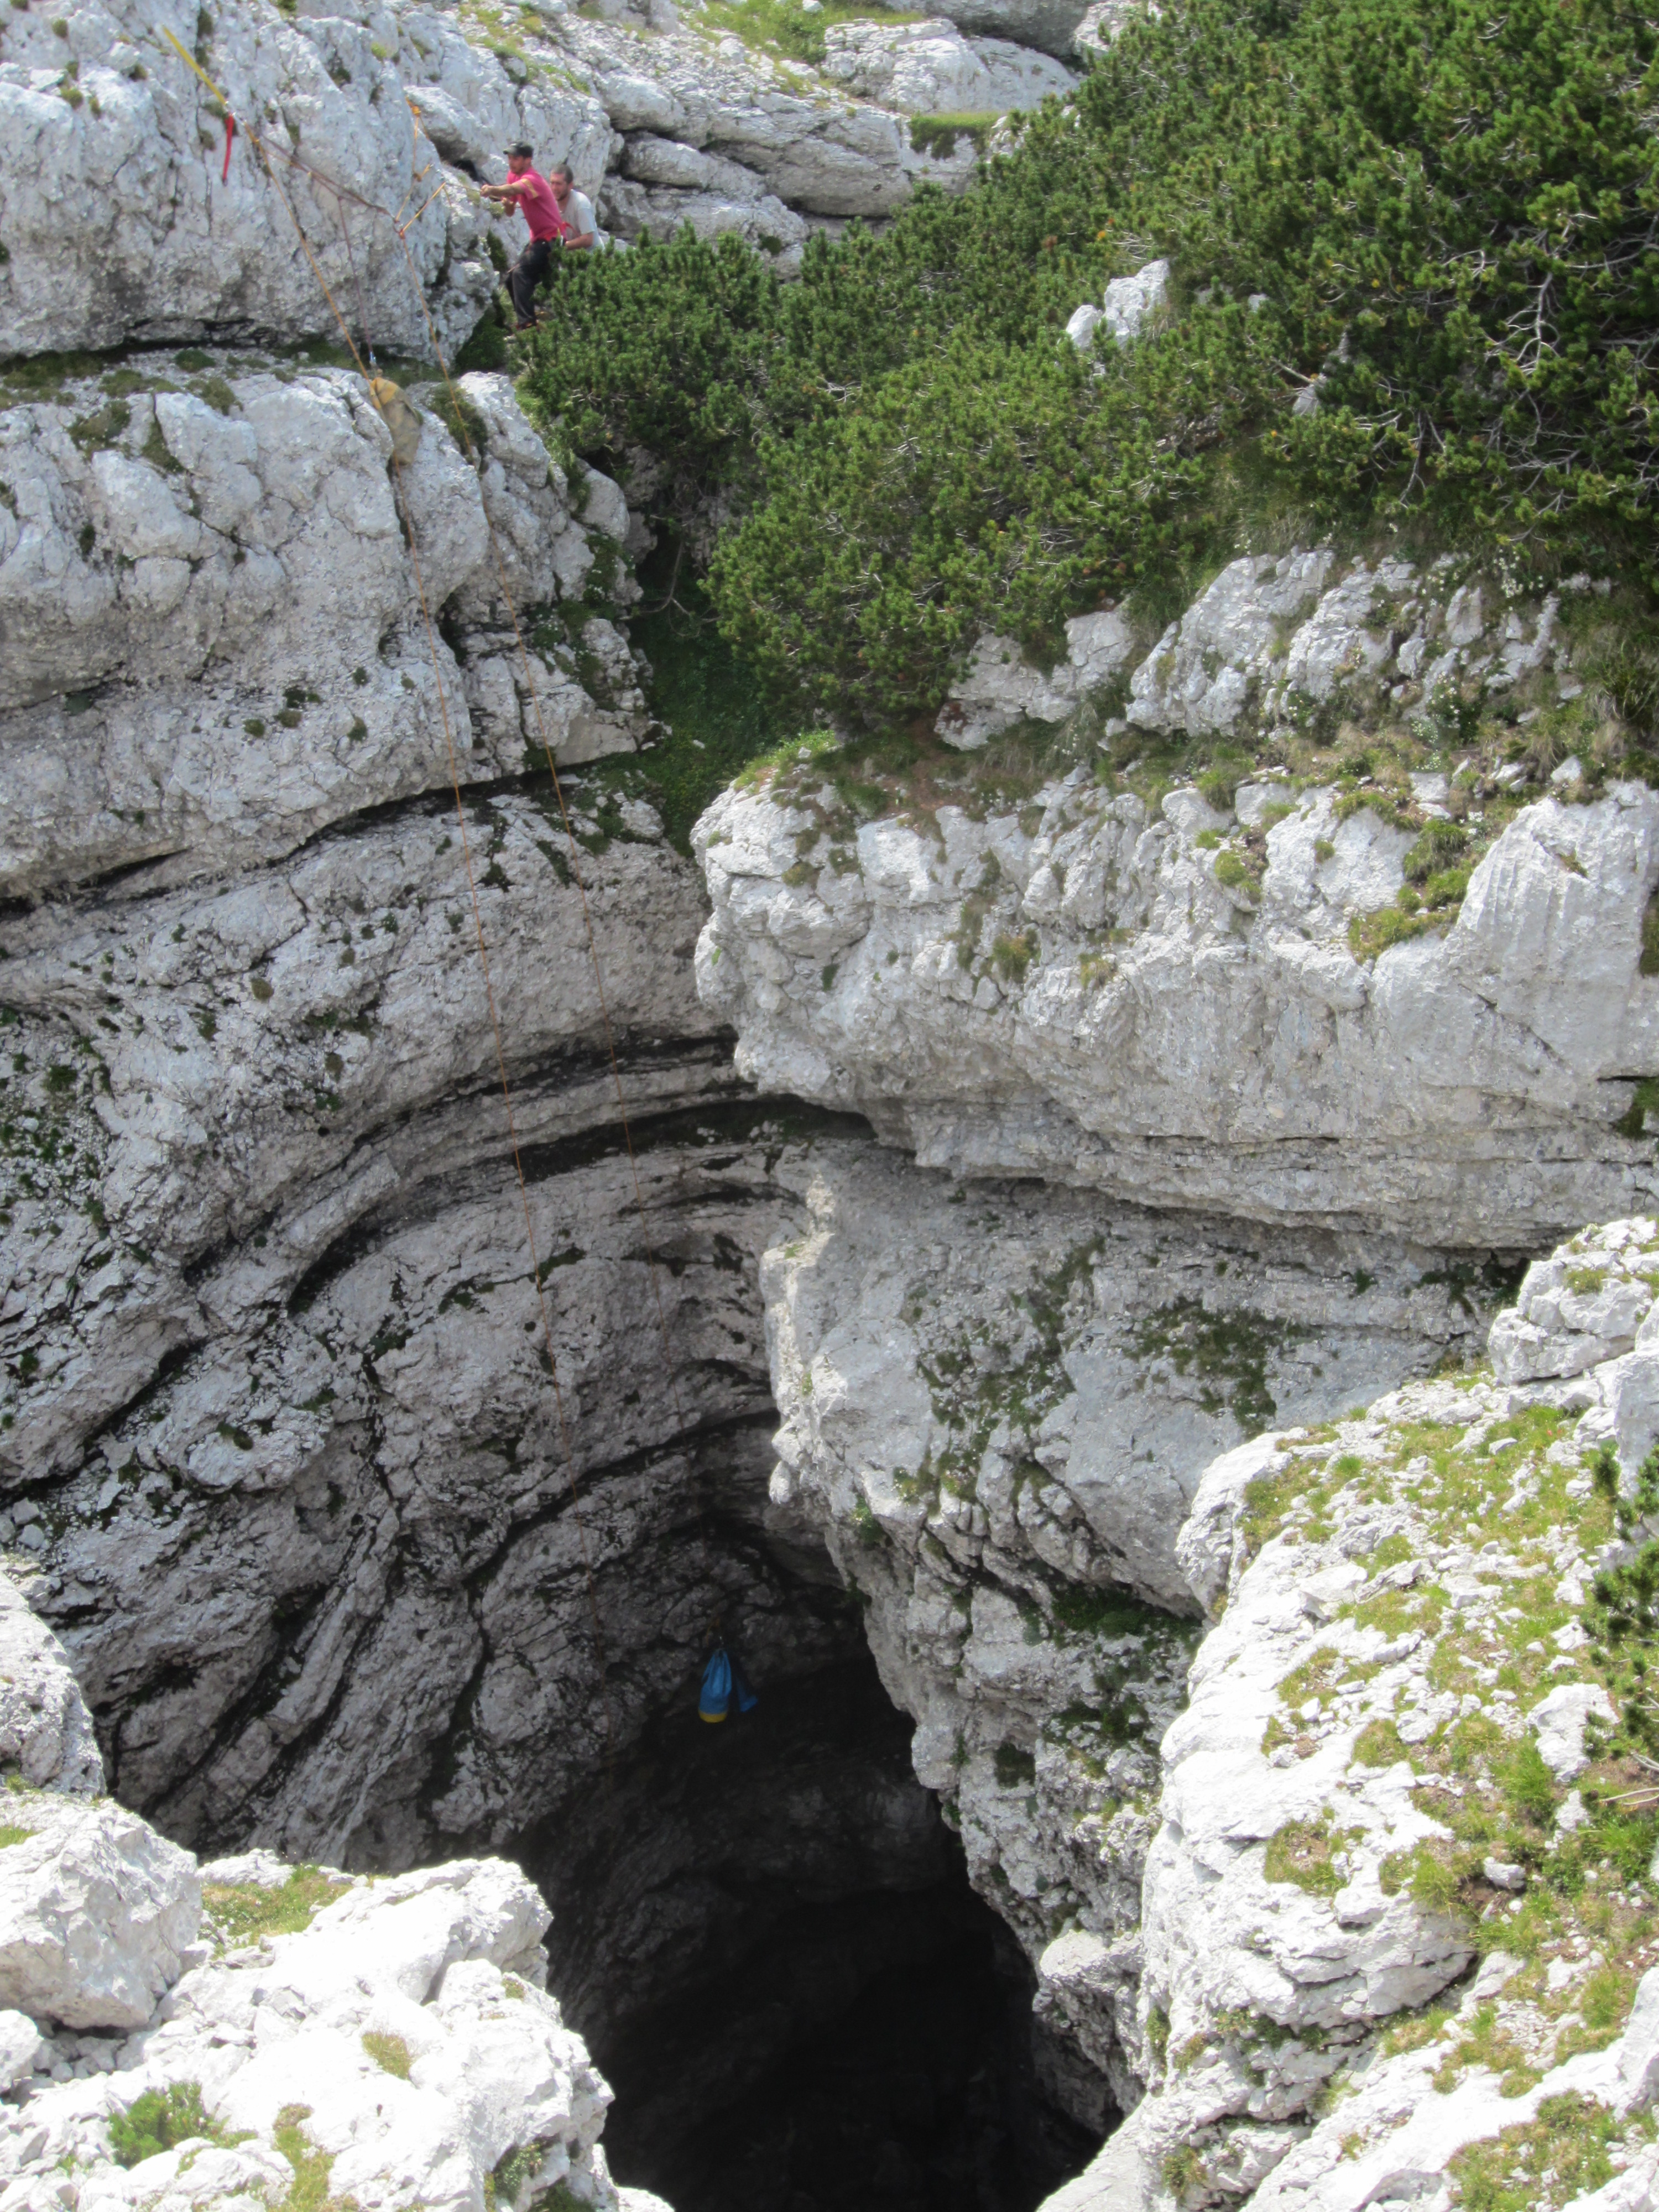
\includegraphics[height=\paperheight]{2012/intro/2012-07-30-2236-TharatornSupasiti-IMG_0126--orig.jpg}}
}
\BgThispage









